\documentclass[twoside,twocolumn]{article}

\usepackage{blindtext} % Package to generate dummy text throughout this template 
\usepackage{graphicx}
\usepackage[sc]{mathpazo} % Use the Palatino font
\usepackage[T1]{fontenc} % Use 8-bit encoding that has 256 glyphs
\linespread{1.05} % Line spacing - Palatino needs more space between lines
\usepackage{microtype} % Slightly tweak font spacing for aesthetics

\usepackage[english]{babel} % Language hyphenation and typographical rules

\usepackage[hmarginratio=1:1,top=32mm,columnsep=20pt]{geometry} % Document margins
\usepackage[hang, small,labelfont=bf,up,textfont=it,up]{caption} % Custom captions under/above floats in tables or figures
\usepackage{booktabs} % Horizontal rules in tables
\usepackage{graphicx}
\usepackage{lettrine} % The lettrine is the first enlarged letter at the beginning of the text

\usepackage{listings}
\usepackage{color}

\definecolor{dkgreen}{rgb}{0,0.6,0}
\definecolor{gray}{rgb}{0.5,0.5,0.5}
\definecolor{mauve}{rgb}{0.58,0,0.82}

\lstset{frame=tb,
  language=SQL,
  aboveskip=3mm,
  belowskip=3mm,
  showstringspaces=false,
  columns=flexible,
  basicstyle={\small\ttfamily},
  numbers=none,
  numberstyle=\tiny\color{gray},
  keywordstyle=\color{blue},
  commentstyle=\color{dkgreen},
  stringstyle=\color{mauve},
  breaklines=true,
  breakatwhitespace=true,
  tabsize=3
}

%\usepackage{minted}

\usepackage{enumitem} % Customized lists
\setlist[itemize]{noitemsep} % Make itemize lists more compact

\usepackage{abstract} % Allows abstract customization
\renewcommand{\abstractnamefont}{\normalfont\bfseries} % Set the "Abstract" text to bold
\renewcommand{\abstracttextfont}{\normalfont\small\itshape} % Set the abstract itself to small italic text

\usepackage{titlesec} % Allows customization of titles
\renewcommand\thesection{\Roman{section}} % Roman numerals for the sections
\renewcommand\thesubsection{\roman{subsection}} % roman numerals for subsections
\titleformat{\section}[block]{\large\scshape\centering}{\thesection.}{1em}{} % Change the look of the section titles
\titleformat{\subsection}[block]{\large}{\thesubsection.}{1em}{} % Change the look of the section titles

\usepackage{fancyhdr} % Headers and footers
\pagestyle{fancy} % All pages have headers and footers
\fancyhead{} % Blank out the default header
\fancyfoot{} % Blank out the default footer
\fancyhead[C]{Estructuras de datos en bases de datos $\bullet$ Octubre 2020 $\bullet$ } % Custom header text
\fancyfoot[RO,LE]{\thepage} % Custom footer text

\usepackage{titling} % Customizing the title section

\usepackage{hyperref} % For hyperlinks in the PDF

%----------------------------------------------------------------------------------------
%	TITLE SECTION
%----------------------------------------------------------------------------------------

\setlength{\droptitle}{-4\baselineskip} % Move the title up
 % Article title formatting
 % Article title closing formatting
\title{Beneficios y perjuicios de la utilización de estructuras de datos en bases de datos relacionales } % Article title
\author{Derian Herrera, Julio Mejia, Randi Paredes , Abraham Lipa}
\date{\today} % Leave empty to omit a date
\renewcommand{\maketitlehookd}{%

}

%----------------------------------------------------------------------------------------

\begin{document}

% Print the title
\maketitle

%----------------------------------------------------------------------------------------
%	ARTICLE CONTENTS
%----------------------------------------------------------------------------------------

\section{Resumen}

\lettrine[nindent=0em,lines=3]{E}n el presente articulo estaremos explicando lo que es una base de datos relacional cuales son las partes que la conforman así como también daremos a conocer sobre las estructura de datos y el impacto tanto bueno como malo que traen estos al momento de implementarlo en una base de datos relacional. Nos enfocaremos en la estructura de datos tipo árbol dando a saber su estructura y su implementación.



%------------------------------------------------

\section{Abstract}


In this article we will be explaining what a relational database is, which are the parts that make it up, as well as we will make known about the data structure and the good and bad impact that these bring when implementing it in a database. real data. 
We will focus on the tree-like data structure giving its structure and implementation.






%------------------------------------------------
\section{Introduccion}
Antes de iniciar con el desarrollo primero veremos el concepto de una base de datos.
Una base de datos es un conjunto de datos almacenados en memoria externa que están organizados mediante una estructura de datos. Cada base de datos ha sido diseñada para satisfacer los requisitos de información de una empresa u otro tipo de organización, como por ejemplo, una universidad o un hospital.
Una base de datos se puede percibir como un gran almacén de datos que se define y se crea una sola vez, y que se utiliza al mismo tiempo por distintos usuarios. [1]
Estas base de datos necesitan de un gestor de base de datos o también llamado SGBD es una aplicación que permite a los usuarios definir, crear y mantener la base de datos, además de proporcionar un acceso controlado a la misma. Se denomina sistema de bases de datos al conjunto formado por la base de datos, el SGBD y los programas de aplicación que dan servicio a la empresa u organización. [1]
Luego de conocer estos conceptos entraremos al tema central el cual es la base de datos relacionales y de las estructuras que pueden tomar junto con sus ventajas y desventajas.

\section{Desarrollo}

\subsection{Base de datos relacional}
La base de datos relacionales o modelo relacional 
fue definido por Edgar Frank Codd a finales de los años
60; en 1970 publicaría un documento que llevaba por nombre
A Relational Model of data for Large Shared Data Banks 
(Un modelo relacional de datos para grandes bancos de datos compartidos), 
siendo este el documento más importante sobre esta materia y del cual nace el término. El modelo relacional es el más utilizado en la actualidad.[2]
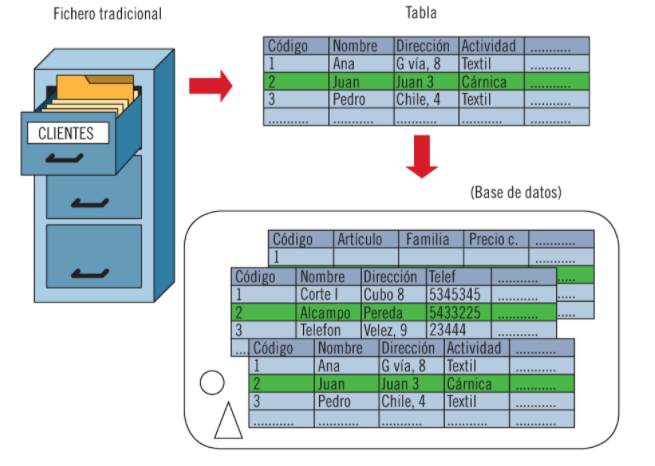
\includegraphics[width=7cm, height=7cm]{img/base de datos relacional.png}
\begin{itemize}
\item  \textbf{Concepto }
Una base de datos relacionales es aquella que
representa los datos y las relaciones entre los
datos mediante una colección de tablas, cada una
con un nombre único, donde una fila de una tabla 
representa una relación entre un conjunto de valores.[2]
\item  \textbf{Ejemplificación}
Los principales objetivos perseguidos por 
Edgar Codd sobre el modelado de datos relacional son los siguientes: 
\textbf{-Independencia física.} La forma de almacenar los datos no debe afectar en su manipulación lógica.
\textbf{Independencia lógica.} Las aplicaciones utilizadas en la base de datos no deben ser modificadas al cambiar elementos de la base de datos. 
\textbf{Flexibilidad.} Los datos se pueden presentar a los usuarios de manera que se puedan adaptar a sus necesidades. 
\textbf{Uniformidad.} La organización de los datos tendrá siempre la misma estructura lógica, usando valores explícitos que contienen las relaciones (las tablas). [3]

\end{itemize}

Luego de ver que es una base de datos relacional pasaremos a explicar un poco de las estructuras de datos.
Una estructura de datos  es una  agregación  de tipos  de datos  compuestos  y atómicos  en un conjunto  con relaciones  bien definidas , Una estructura  significa  un conjunto  de reglas  que contienen los datos juntos. [3]
Lo que se quiere decir es 	que una estructura de datos es una forma particular de organizar datos en una computadora para que puedan ser utilizados de manera eficiente. Son un medio para manejar grandes cantidades de datos eficientemente.
Una elección inadecuada de la estructura de datos puede conducir a programas lentos, largos y poco eficientes.
Una solución se denomina eficiente si resuelve el problema dentro de las restricciones de recursos requeridas. Restricciones de recursos pueden ser el espacio total disponible para almacenar los datos o el tiempo permitido para ejecutar cada subtarea. Se suele decir que una solución es eficiente cuando requiere menos recursos que las alternativas conocidas.

\subsection{Estructuras de datos en Bases de datos}
Los estructuras de datos son ampliamente usadas en el funcionamiento interno de la mayoría de los motores SQL. Específicamente en la organización de los índices, para los cuales se usa un tipo de árbol conocido como B-tree. [5]


La estructura de los índices manejada en B-Trees puede cambiar ligeramente según la cantidad de CPUs que son usados para crear y reconstruir los índices, pero para la mayor parte, el tamaño y la extensión de un arbol está basado en la definición de el índice y la cantidad de registros en la tabla.[5]


Sin embargo, la implementación de una estructura de datos para almacenar datos que posteriormente queremos utilizar para realizar consultas de busqueda (por ejemplo), puede resultar interesante según sus resultados.

\subsection{Árboles generales}
Un arbol en general es una estructura de datos que almacena elementos jerarquicamente, los elementos en un arbol se suelen llamar nodos. Con la excecpción del primer elemento de arriba, cada elemento en el arbol tiene uno o más hijos. Por tanto, la relación entre padres e hijos se daría de arriba hacía abajo. Son no lineares porque sus elementos no tiene una relación simple de "antes" y "después", más bien se podría referir a las relaciones como "de padre a hijo" y como a sus elementos "ancestros" y "descendientes".[4]

\subsection{Arboles binarios}
Un arbol binario es una arbol ordenado que tiene las siguientes propiedades [4]:

\begin{enumerate}
  \item Cada nodo (o elemento) tiene a lo mucho dos hijos
  \item Cada nodo hijo es etiquetado como hijo izquierdo o hijo derecho
  \item Un hijo izquierdo precede al hijo izquierdo en el orden de los hijos de un nodo
\end{enumerate}

Esta es la implementación más simple de un arbol binario en el que solo se usan los números como identificadores, sin embargo, también se pueden utilizar otros tipos de datos como cadenas de texto. El tipo de dato elegido debe tener un criterio de ordenamiento para poder ser usado efectivamente.

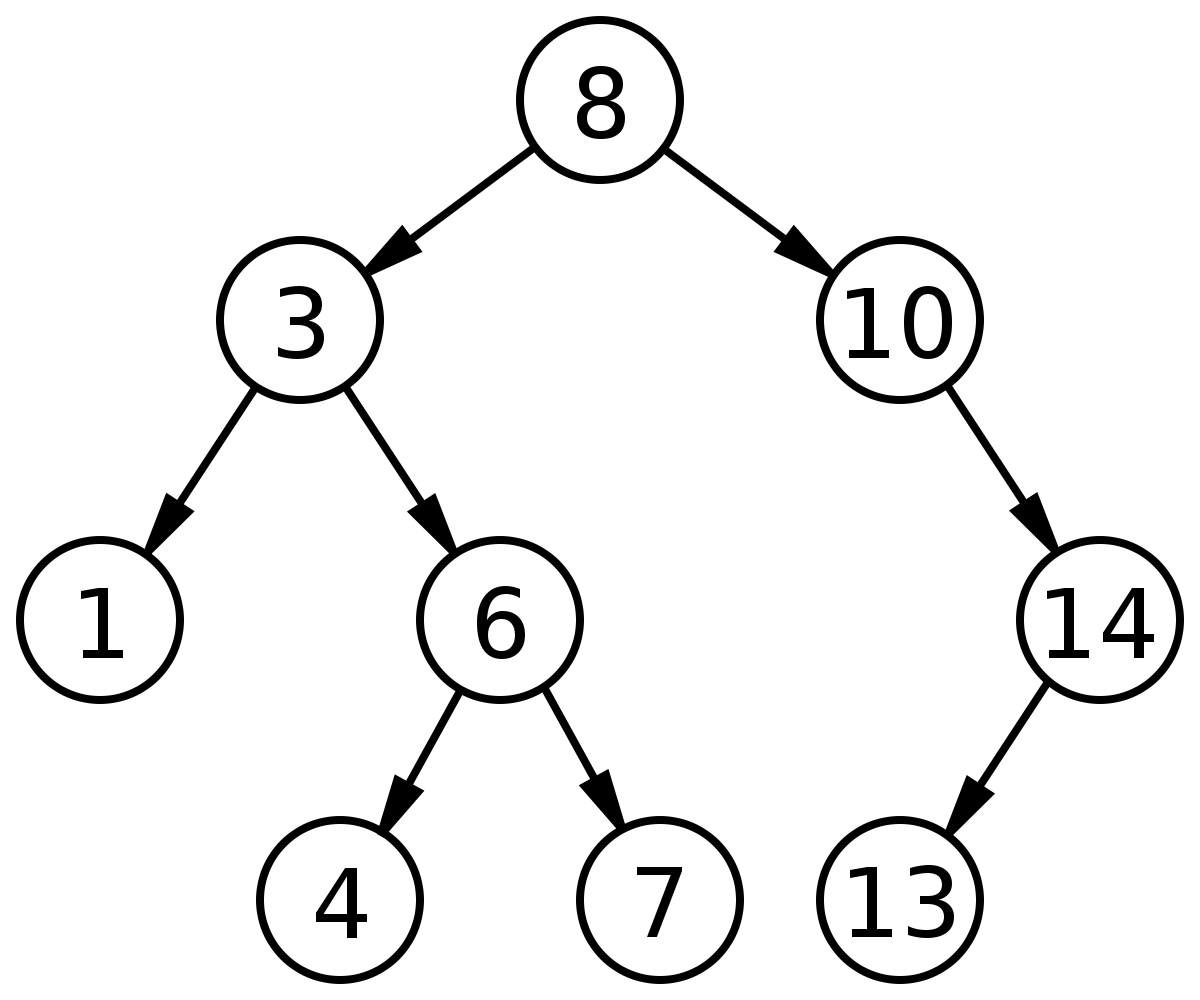
\includegraphics[width=7cm, height=6cm]{img/1200px-Binary_search_tree.svg}

Algunas de las operaciones que se pueden realizar sobre los arboles binarios de búsqueda son el pre-orden y el post-orden.

\subsubsection{Algoritmos transversales}

Los algoritmos transversales son formas sistemáticas de acceder a todos los elementos del arbol. [6]
A continuación, se describiran dos de estos algoritmos.

\subsubsection{Pre-orden}

Mediante este algoritmo, la raiz del arbol es visitada primero y luego los sub-arboles hijos son visitados recursivamente. En el caso de que sea un arbol ordenado, los sub-arboles son accedidos de acuerdo al orden de los hijos. [6]
Para recorrer un árbol binario no vacío en preorden, hay que realizar las siguientes operaciones recursivamente en cada nodo, comenzando con el nodo de raíz:

\begin{enumerate}
  \item Visite la raíz
  \item Atraviese el sub-árbol izquierdo
  \item Atraviese el sub-árbol derecho
\end{enumerate}

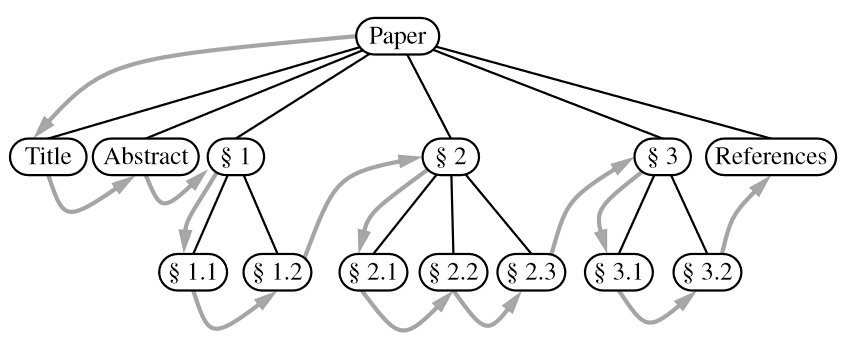
\includegraphics[width=7cm, height=3cm]{img/Screenshot_2.png}

\subsubsection{In-orden}

Mediante este algoritmo, el sub-arbol izquierdo es visitado recursivamente primero, luego la raiz del arbol y finalmente, el sub-arbol derecho es visitado recursivamente . En el caso de que sea un arbol ordenado, Todos los elementos del arbol son accedidos según el criterio de ordenamiento. [6]
Para recorrer un árbol binario no vacío en preorden, hay que realizar las siguientes operaciones recursivamente en cada nodo, comenzando con el nodo de raíz:

\begin{enumerate}
  \item Atraviese el sub-árbol izquierdo
  \item Visite la raíz
  \item Atraviese el sub-árbol derecho
\end{enumerate}

\subsubsection{Post-orden}

Generalmente, este algoritmo es considerado el opuesto del Pre-orden. Mediante este algoritmo, los sub-arboles hijos son visitados recursivamente y luego la raiz del arbol es visitada. [6]
Para recorrer un árbol binario no vacío en inorden (simétrico), hay que realizar las siguientes operaciones recursivamente en cada nodo:

\begin{enumerate}
  \item Atraviese el sub-árbol izquierdo
  \item Atraviese el sub-árbol derecho
  \item Visite la raíz
\end{enumerate}

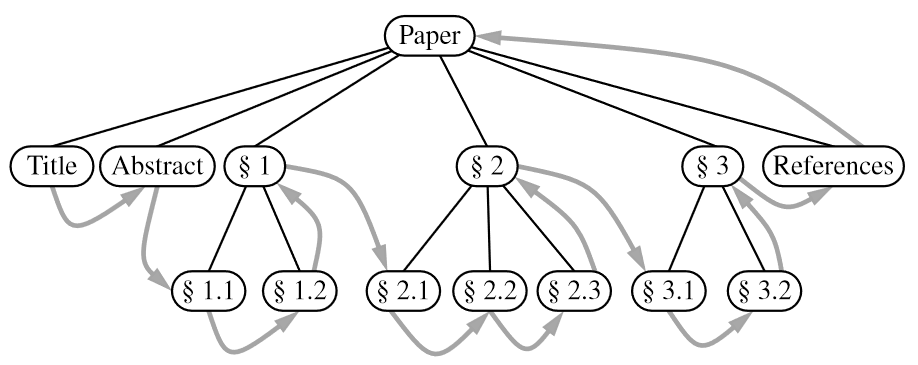
\includegraphics[width=7cm, height=3cm]{img/Screenshot_3.png}

\subsubsection{Aplicaciones frecuentes}

Entre las aplicaciones frecuentes, se encuentran implementaciones sobre datos que están en una jeraquía. [6]

Una aplicación clásica de los arboles binarios es la tabla de contenidos o índice. Dado que cada elemento de una tabla de contenidos está jerarquizado, se podría generar naturalmente un índice mediante el algoritmo de pre-orden. Se pueden obtener mejores resultados considerando la profundidad en la identación de los elementos. [6]

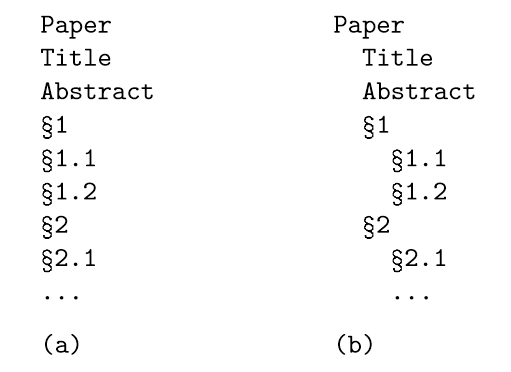
\includegraphics[width=7cm, height=5cm]{img/Screenshot_4.png}

\subsection{Implementación en Bases de datos}
La implementación de una estructura de árbol en bases de datos directamente sobre el alamacenamiento de los datos, se puede aplicar mediante la siguiente estructura que corresponde a un arbol binario. En este caso hemos utilizado T-SQL.

\begin{lstlisting}
CREATE TABLE Binary_Tree (
  node_id INTEGER NOT NULL PRIMARY KEY,
  parent_node_id INTEGER NOT NULL,
   CHECK (parent_node_id <> node_id),
  node_flag CHAR(1) DEFAULT 'L' NOT NULL
   CHECK (node_flag IN ('L', 'R'))
  user_first_name VARCHAR(25) NOT NULL);
\end{lstlisting}

Aunque esta estructura es válida y es posible crear nodos que formen parte del arbol binario, no puede funcionar correctamente debido a que no existen suficientes restricciones para el registro de los datos. Por ejemplo, no tenemos restricciones para ejecutar la siguiente instrucción.

\begin{lstlisting}
 INSERT INTO Binary_Tree
 VALUES (1, 2, 'L', 'Sam'),
        (1, 3, 'R', 'Fred'),
        (3, 4, 'L', 'John'),
        (4, 1, 'L', 'Loop');
\end{lstlisting}

Para evitar estos casos, se podrían agregar restricciones para la cantidad de hijos de un nodo y la cantidad de hijos izquierdos y derechos (que deben ser uno de cada uno).

\begin{lstlisting}
 NOT EXISTS
 (SELECT node_id
    FROM Binary_Tree
   GROUP BY node_id
  HAVING COUNT(*) > 2)

 NOT EXISTS
 (SELECT node_id
    FROM Binary_Tree
   GROUP BY node_id
  HAVING SUM(CASE WHEN node_flag = 'L'
         THEN 1 ELSE 0 END) > 1
     OR SUM(CASE WHEN node_flag = 'R'
         THEN 1 ELSE 0 END) > 1)
\end{lstlisting}

Con la implementación de estas restricciones tendríamos control sobre los registros insertados en la tabla.


\subsection{Beneficios}
Uno de los beneficios más importantes de una estructura de datos como el arbol binario específicamente de búsqueda, es que requiere menos accesos al árbol al realizar una búsqueda.

En el peor de los casos, se tendría una estructura de datos similar a una lista enlazada. Esto sucede cuando el árbol es degenerado y cada nodo solo tiene o un hijo izquierdo o un hijo derecho.

Pero si se logra equilibrar el árbol de manera que tenga una cantidad similar de nodos en cada lado del árbol completo, resulta teniendo mejores resultados que recorrer los registros de uno a uno.


\subsection{Perjuicios}
El principal perjuicio que tiene la implementación de esta estructura de datos es el tiempo que toma el reordenamiento de nuevos registros al ser insertados en el árbol o de registros que son actualizados.

Se tienen que realizar muchos cambios dependiendo del orden del dato que queramos ingresar. En el peor de los casos puede tardar notablemente más que una inserción o modificación regular.
       
\section{Conclusiones}

El modelo relacional para bases de datos se caracteriza por la claridad, tiene una base matemática y ha probado su eficacia en la práctica durante más de 40 años. Pese a todo, el almacenamiento de datos en tablas estructuradas no se ha adaptado a las necesidades de la tecnología de la información moderna.

Son especialmente la gestión de grandes volúmenes de datos en el marco de los análisis de big data y el almacenamiento de datos abstractos los factores que saturan la capacidad de los sistemas relacionales. Y es precisamente aquí donde los sistemas especializados, como las BD basadas en objetos o los conceptos desarrollados en la senda del movimiento NoSQL, muestran su superioridad, si bien no es posible prescindir completamente del modelo relacional. Las bases de datos relacionales despliegan todo su potencial sobre todo en aquellos ámbitos corporativos protagonizados por el procesamiento de datos de transacciones.

Los datos sobre acciones de los clientes o medidas de marketing pueden representarse perfectamente en el formato de tabla, a la par que los usuarios sacan provecho de una sintaxis que, pese a su simplicidad, permite consultas complejas.

\section{Recomendaciones}

Las siguientes recomendaciones son solamente algunas de las muchas que se deben considerar para mantener la seguridad en una base datos y este es un manual para el diseño y implementación de una base de datos. A continuación, se enumeran las recomendaciones junto con una breve explicación:

\begin{itemize}
\item El administrador de la base datos es el único que debe tener acceso a la base de datos.
\item El administrador de la base de datos es quién se encarga de ingresar los SQL, se recomienda utilizar una base datos a escala de la base de datos principal para verificar la eficiencia de las sentencias SQL en esta base antes de ingresarlos en la base de datos principal.
\item Solo los administradores de la base de datos deben tener acceso a la documentación de la misma.
\item Cuando se realiza algún cambio en la base de datos a nivel físico, lógico o en el modelo de datos dicho cambio debe ser actualizado en la documentación de la misma, esto con el fin de que la documentación siempre este actualizada.
\item Finalmente, como última recomendación es importante fomentar el uso de sentencias SQL optimizadas
\end{itemize}


\begin{thebibliography}{99} % Bibliography - this is intentionally simple in this template

\bibitem
[1].Marqués, M. (2009). Bases de datos. Castelló de la Plana, Spain: D - Universitat Jaume I. Servei de Comunicació i Publicacions. 
\bibitem
[2].Jiménez Capel, M. Y. (2015). Bases de datos relacionales y modelado de datos (UF1471). Antequera, Málaga, Spain: IC Editorial.
\bibitem
[3].Zohonero Martínez, I. y Joyanes Aguilar, L. (2008). Estructuras de datos en Java. Madrid etc, Spain: McGraw-Hill España.
\bibitem
[4].Goodrich, M. T., Tamassia, R., \& Mount, D. M. (2011). Data Structures and Algorithms in C++ (2nd ed.). Wiley.
\bibitem
[5].Delaney, K., Beauchemin, B., Cunningham, C., Kehayias, J., Randal, P. S., \& Nevarez, B. (2013). Microsoft SQL Server 2012 Internals (Developer Reference) (1st ed.). Microsoft Press.
\bibitem
[6].Goodrich, M. T., Tamassia, R., \& Goldwasser, M. H. (2013). Data Structures and Algorithms in Python (1st ed.). Wiley.
\end{thebibliography}

%----------------------------------------------------------------------------------------

\end{document}